\chapter{Introduction}
What and where is dark matter? For a question so central to cosmology and particle physics, the prospects for finding an answer do not at first glance seem promising. As with so many things in physics, we should not by all rights be able to answer the question, nature having hidden itself away in the dark recesses of the universe. But dark matter is all around us and we merely need a window through which to view it. In this work, I will discuss strategies for the direct detection of dark matter: how they offer us a window - however murky - into the dark universe; how they are faced with myriad  uncertainties; and how those uncertainties can be overcome to help us to understand more about what dark matter is and how it is distributed in our tiny patch of the universe.

The question `\textit{What is dark matter?}' is perhaps best answered by reviewing the current evidence for its existence. Evidence for dark matter is found on scales from the Milky Way up to the cosmological horizon, with a range of observations which cannot be adequately explained with the observed constituents of the universe. Dark matter is an invisible component introduced to reconcile these observations with the known laws of physics - most importantly, General Relativity. Beyond this general definition, there are a wide range of particle physics candidates which may play the role of dark matter. These typically derive from theories of physics beyond the Standard Model, meaning that the study of the properties of dark matter can shed light on theories of high energy physics. Many of these proposed dark matter candidates have weak but non-zero interactions with particles of the Standard Model, leading to several avenues through which it is hoped the non-gravitational detection of dark matter may soon be achieved.

In this chapter, we summarise the evidence in support of the dark matter paradigm, including constraints from precision cosmology. We then describe some of the broad classes into which particle dark matter candidates can be categorised, as well as describing a few specific candidates in more detail. Finally, we discuss current progress and constraints from direct and indirect searches for particle dark matter.

\section{Evidence for dark matter}

Dark matter is a key component of the \LCDM paradigm of modern cosmology. In this framework, the energy density of the universe today is dominated by the constant and uniform contribution of the vacuum, $\Lambda$, also referred to as Dark Energy. This contribution exerts a negative pressure and drives the accelerating expansion of the universe which was the subject of the 2011 Nobel Prize in Physics \cite{Riess:1998, Perlmutter:1999}. However, the formation of structure in the early universe is driven by the clustering of an inert, slow moving and as yet undetected matter component \cite{Kolb:1990}: Cold Dark Matter. In \LCDM cosmology, baryonic matter makes up a much smaller fraction of the energy density of the universe. Cosmological experiments allow us to precisely determine the contributions of these various components (see e.\ g.\  WMAP \cite{Hinshaw:2013}, BOOMERanG \cite{MacTavish:2005}, BOSS \cite{Dawson:2013}, BICEP2 \cite{Ade:2014} and CFHTLenS \cite{Kitching:2014} to name just a few.)

A particularly sensitive probe for determining the dark matter contribution to the energy budget of the universe is the measurement of the temperature anisotropies of Cosmic Microwave Background (CMB) photons. These contain an imprint of the acoustic oscillations of the baryon-photon fluid during the era of recombination. The scale of these oscillations is sensitive to the size of the gravitational potential generated in the early universe by dark matter. \note{This is shite and needs fixing, am I talking about BAOs or what?} The recent Planck experiment \cite{PlanckI:2013} measured the angular power spectrum of these CMB temperature anisotropies. Figure~\ref{fig:intro:CMB} shows the results of these measurements, as well as the best fit 6-parameter \LCDM model. The contribution of the cosmological constant, the total matter component, and the separate baryonic and dark matter components to the total energy density of the universe is shown in Table~\ref{tab:intro:Planck}, constrained with an accuracy of less than 3\%. We are lead to the conclusion that $\sim$84\% of the matter content of the universe is in fact dark.

\todo{Read for details: arXiv:1404.5415}

\note{CFHTLENS: arXiv:1404.5469}

\begin{figure}[h]
  \label{fig:intro:CMB}
  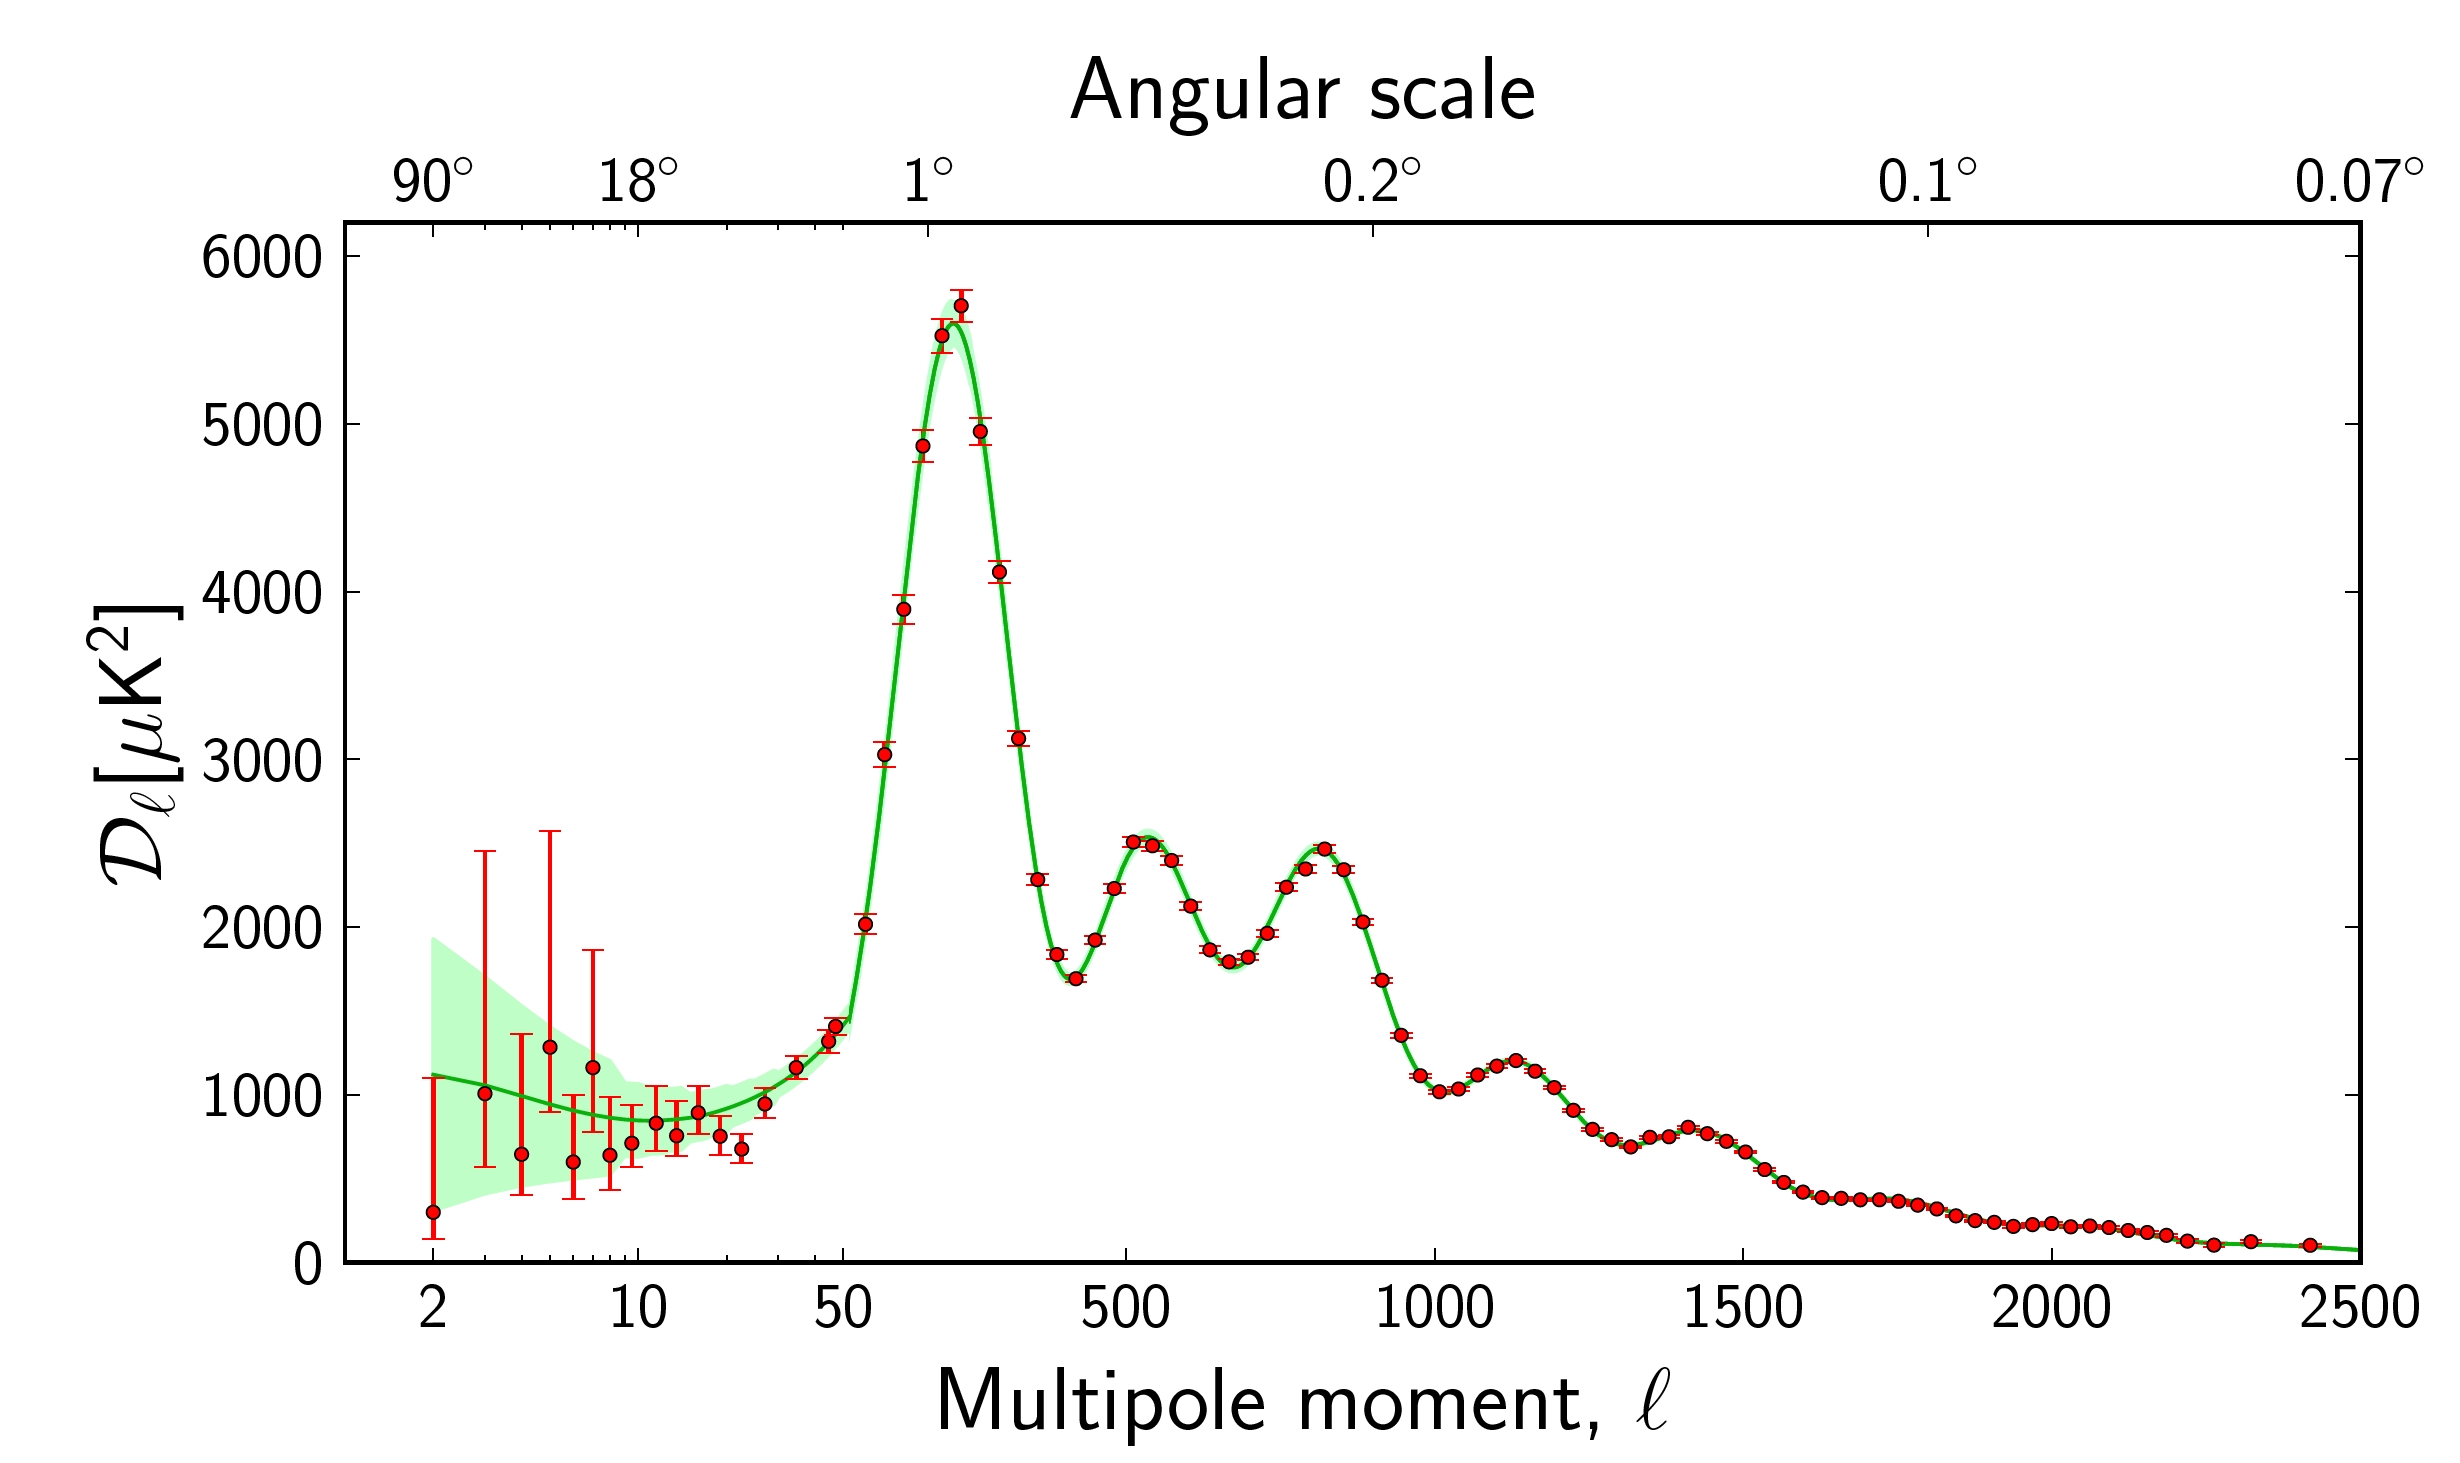
\includegraphics[width=\textwidth]{CMBanisotropies.jpg}
  \caption[CMB anisotropies measured by the Planck experiment]{CMB anisotropies. \note{Need actual caption}}
\end{figure}


\begin{table}
  \begin{center}
	\begin{tabular}{cc}
        \hline\hline
        Parameter & 68\% limits \\
        \hline
        $\Omega_\Lambda$ & 0.686 $\pm$ 0.020 \\
        $\Omega_m h^2$ & 0.1423 $\pm$ 0.0029 \\
        $\Omega_b h^2$ & 0.02207 $\pm$ 0.00033 \\
        $\Omega_c h^2$ & 0.1196 $\pm$ 0.0031 \\
        \hline\hline
	\end{tabular}
  \end{center}
  \caption[Cosmological parameters obtained by the Planck Collaboration]{Energy density of the cosmological constant ($\Lambda$), total matter ($m$), and separate baryonic ($b$) and cold dark matter ($c$) components in units of the critical density \note{define...}, as obtained by the Planck Collaboration \cite{PlanckXVI:2013}. The Hubble parameter is defined as $H_0 = 100 \,\,h \, \textrm{km s}^{-1} \textrm{Mpc}^{-1}$.}
  \label{tab:intro:Planck}
\end{table}

However, the evidence for dark matter is not purely cosmological. In 1933, Zwicky measured the velocity dispersion of galaxies in the Coma cluster \cite{Zwicky:1933}. An application of the Virial Theorem indicated a gravitational mass in the cluster which was several hundred times bigger than that expected from the luminosity of the member galaxies. It is now known that some of this mass is in the form of hot ($\sim$1 million K), X-ray emitting intracluster gas \cite{Sanders:2013}. Nonetheless, a discrepancy remains; current estimates of the mass-to-light ratio of the Coma cluster give a value of roughly 150 times that of the Sun \cite{Fusco-Femiano:1994,Makino:1994}. However, the Coma cluster does not appear to be unusual. Measurements of the masses of a large number of galaxy clusters using gravitational lensing \cite{Okabe:2013}, X-ray observations \cite{Ettori:2013} and dynamical estimates \cite{Carlberg:1995} indicate that a significant fraction of a cluster's mass must be dark.

The validity of the \LCDM paradigm is also borne out in results from N-body simulations. These simulations track the evolution of structure in the universe by accounting for the dynamics and gravitational interactions \note{only Newtonian?} of a large number of particles starting from some initial conditions. These may be horizon-scale cosmological simulations, tracing the collapse of the initial density perturbations after decoupling (such as the the Millenium simulation \cite{Springel:2005}), or galaxy-scale simulations, tracing the formation and growth of a small number of galaxies starting from initial conditions at intermediate redshift (such as the Via Lactea \cite{Diemand:2006} and Aquarius \cite{Springel:2008} simulations).

\note{Maybe swap this paragraph with the next one - it makes more sense?} A variety of sophisticated computational techniques (such as smoothed particle hydrodynamics \cite{Stinson:2010}, adaptive mesh refinement \cite{Norman:1999} and moving mesh cosmology \cite{Springel:2010}) have been employed and refined to make such simulations computationally feasible and to allow higher and higher resolutions to be reached. In spite of this, computational limitations mean that the highest resolution simulations still use `particle' masses of the order of $10^5 M_{\odot}$ \cite{Pillepich:2014}, many orders of magnitude more massive than the $O$(GeV-TeV) particles expected to make up the universe's dark matter. \note{say more...}

Many N-body simulations are DM-only, simulating only the gravitational dynamics of collisionless particles. However, an increasing number are incorporating baryonic physics such as gas dynamics, as well as stellar evolution, chemical enrichment and a variety of feedback processes \note{Need some citations...}. Appropriately accounting for these factors is extremely complex and in some cases the strength of these processes is unknown and must be tuned in the simulations to match observations (see for example Ref.~\cite{Vogelsberger:2013}). \note{Mention some other problems - shock resolution etc.} Due in part to these difficulties, the impact of baryonic physics on the formation of galaxies and the properties of DM haloes is still uncertain (see for example Refs.~\cite{Martizzi:2012,Pillepich:2014}). I will revisit this topic - and its consequences for the direct detection of dark matter - in Chapter~\ref{ch:DirectDetection}.

In spite of these limitations, a consistent picture has emerged from a vast array of N-body simulations. The size distribution of gravitational structures found in the universe is well matched over a range of distance scales  with that obtained from N-body simulations \note{CITATION!}. In particular, the fact that DM is non-interacting means that it begins to collapse gravitationally earlier in cosmic time than baryonic matter. After decoupling, baryons then fall into the gravitational wells produced by the infalling DM structures. Without DM, the baryonic matter in the universe could not have had enough time to collapse to form the array of gravitationally bound structures we see today \cite{Kolb:1990}. \note{Coldness...}

N-body simulations also suggest that galaxies such as the Milky Way should be embedded in a large, approximately spherical dark matter halo. This is corroborated by observations of the rotation curves of spiral \note{just spirals?} galaxies. In particular, the circular velocity of stars in these galaxies is observed to be approximately constant out to large galactocentric distances \cite{Begeman:1991,Persic:1996}. This is shown schematically in Fig.~\ref{fig:intro:RotationCurves}. \note{Say something about gas, and 21cm emission (so that you can check the rotation beyond the luminous matter). [Optical edge]} The majority of the mass of the luminous disc is concentrated at small radii, suggesting that there should be a Keplerian decay of the circular velocity at large radii: $v \sim r^{-1/2}$. However, the inclusion of a non-luminous dark matter halo can reconcile this expectation with the observed flat rotation curves. The density profiles $\rho(r)$ required to provide a good fit to rotation curve data are consistent with those obtained from N-body simulations, such as the Navarro-Frenk-White profile \note{Is this really true? Cusp/Core problem?}

\begin{equation}
\label{eq:intro:NFW}
\rho(r) = \frac{\rho_0}{r/R_s(1 + r/R_s)^2}\,,
\end{equation}
which is described by the central density $\rho_0$ and a scale radius $R_s$. This provides a good cross-check between the results of N-body simulations, which span scales up to the cosmological, and galactic-scale observations of the local universe. The rotation curve of the Milky Way itself has also been studied \note{[cite Mattia and others self-consistent distribution guys]}, as well as the ultralocal distribution of dark matter near the Sun's position. An understanding of this distribution has significant implications for the study of dark matter detection and we defer a detailed discussion to Chapter~\ref{ch:DirectDetection}.

\begin{figure}[h]
  \label{fig:intro:RotationCurves}
  \centering
  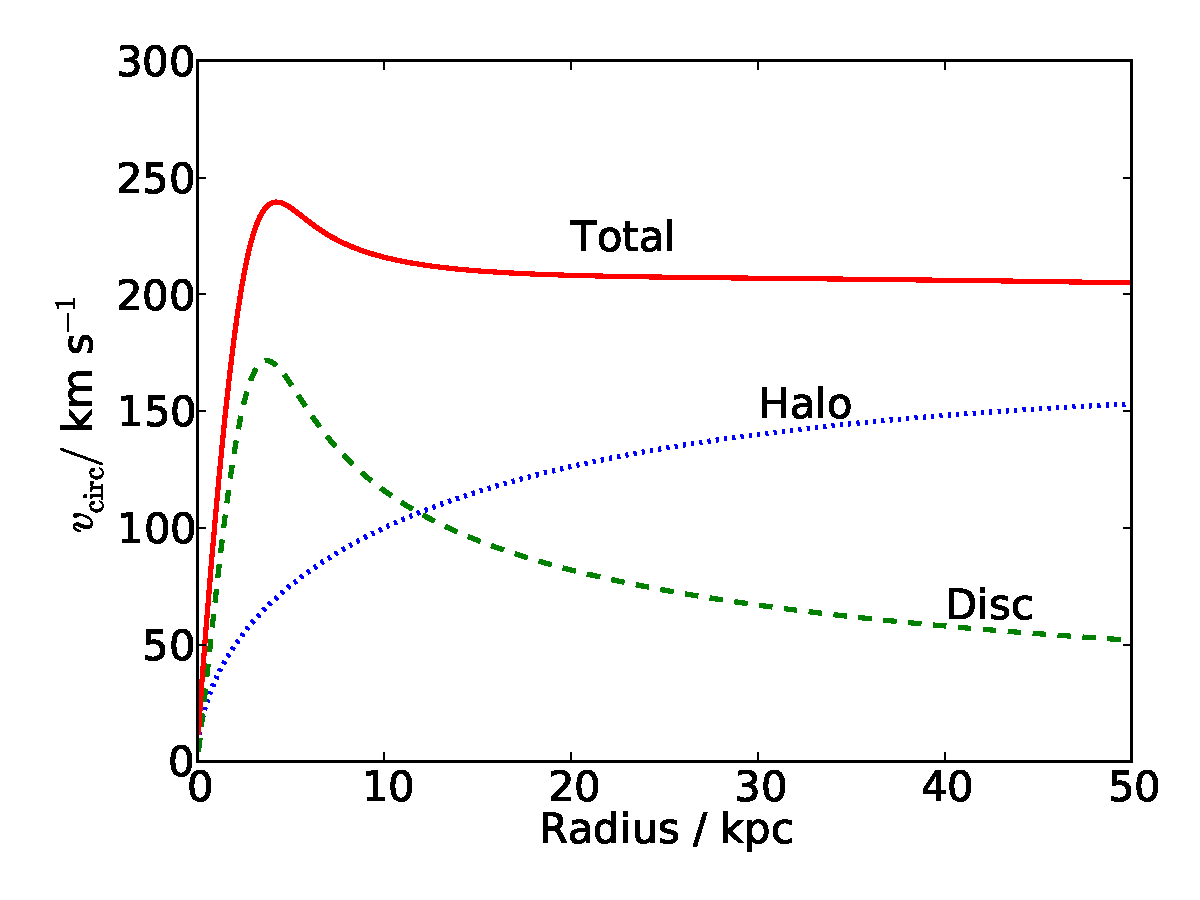
\includegraphics[width=0.8\textwidth]{RotationCurve.pdf}
  \caption[Schematic illustration of galaxy rotation curves]{Schematic illustration of galaxy rotation curves (circular velocity as a function of galactocentric distance). The contribution to the circular velocity from the luminous disc (green dashed line) and dark matter halo (red dotted line) are shown, as well as the total circular velocity (solid blue line). }
\end{figure}



\todo{Need to talk about lensing observations...}
\todo{Nonbaryonic nature determined by primordial nucleosynthesis...}
\todo{Cite Lyndzo!}
\todo{Lensing?}
\todo{Tully-Fisher}

\subsection{Problems with dark matter}

\note{Problems - Too Big to Fail (arXiv:1404.5313); Missing satellites?; Core-Cusp; Identity}

\section{Particle dark matter candidates}

Beyond its gravitational contribution to the universe, we appear to know little about the nature of particle dark matter. However, the success of modern cosmology and the lack of a confirmed detection so far means that we do have a grasp on some of the properties of any potential candidate. Taoso \etal \cite{Taoso:2008} present a `10-point test' which must be passed by any particle before it can be considered as a viable dark matter candidate. Here, I will briefly discuss three of these points, namely, that the DM candidate must be cold, neutral and produced with the appropriate relic density.

\note{Discuss those three conditions - coldness, neutrality and relic density; what about being baryonic; Primordial nucleosynthesis}

The final condition appearing in the `10-point test' of Taoso \etal asks the question `Can it be probed experimentally?' While there are viable DM candidates which interact only gravitationally (such as the gravitino \note{need a ref}), a wide variety of proposed candidates can interact (however weakly) with the particles of the standard model. While the experimental accessibility of a given DM candidate is not a strict necessity, it allows models to be tested (and either falsified or confirmed) beyond the hypothesis stage. In the next section, we explore the different avenues by which models of particle dark matter may be probed.

\section{Detection of dark matter}

\note{Often justified that if it was created in the early universe it should interact with crossing diagrams}
\todo{Do some schematics feynman diagrams for the different detection methods...}



\begin{figure}
\centering
\begin{fmffile}{gluon}
\setlength{\unitlength}{0.1cm}
\begin{fmfgraph}(40,25)
\fmfleft{i1,i2}
\fmfright{o1,o2}
\fmf{fermion}{i1,v1,o1}
\fmf{fermion}{i2,v2,o2}
\fmf{photon}{v1,v2}
\end{fmfgraph}
\end{fmffile}
\begin{fmffile}{gluon2}
\setlength{\unitlength}{0.1cm}
\begin{fmfgraph}(40,25)
\fmfleft{i1,i2}
\fmfright{o1,o2}
\fmf{fermion}{i1,v1,o1}
\fmf{fermion}{i2,v2,o2}
\fmf{photon}{v1,v2}
\end{fmfgraph}
\end{fmffile}
\begin{fmffile}{gluon3}
\setlength{\unitlength}{0.1cm}
\begin{fmfgraph}(40,25)
\fmfleft{i1,i2}
\fmfright{o1,o2}
\fmf{fermion}{i1,v1,o1}
\fmf{fermion}{i2,v2,o2}
\fmf{photon}{v1,v2}
\end{fmfgraph}
\end{fmffile}
\end{figure}



